\section{Conservation}

We expect the following quantities to be physically conserved: mass h, momentum or mass velocity, $hu$ and $hv$, and
energy 0.5($hv^2$+$gh^2$). Potential vorticity is only looked at in the 2D solver. 

\subsection{1D Conservation Laws}
Investigation of conservation laws in the 1D solver shows differences
between the conserved quantities Figure~\ref{fig:1D_cons}. The mass is hypothetically guessed to be strictly conserved by the scheme, 
the momentum should also be strictly conserved by the scheme, unless there are reflections when the walls take
some of the momentum. We observe mass, momentum, and energy to not be conserved adequetly because the inherent nature of 
the numerical schemes ability to capture solutions during shocks.  
\newline

\begin{figure}[h!]
    \centering
    \begin{subfigure}[b]{0.9\textwidth}
        \centering
        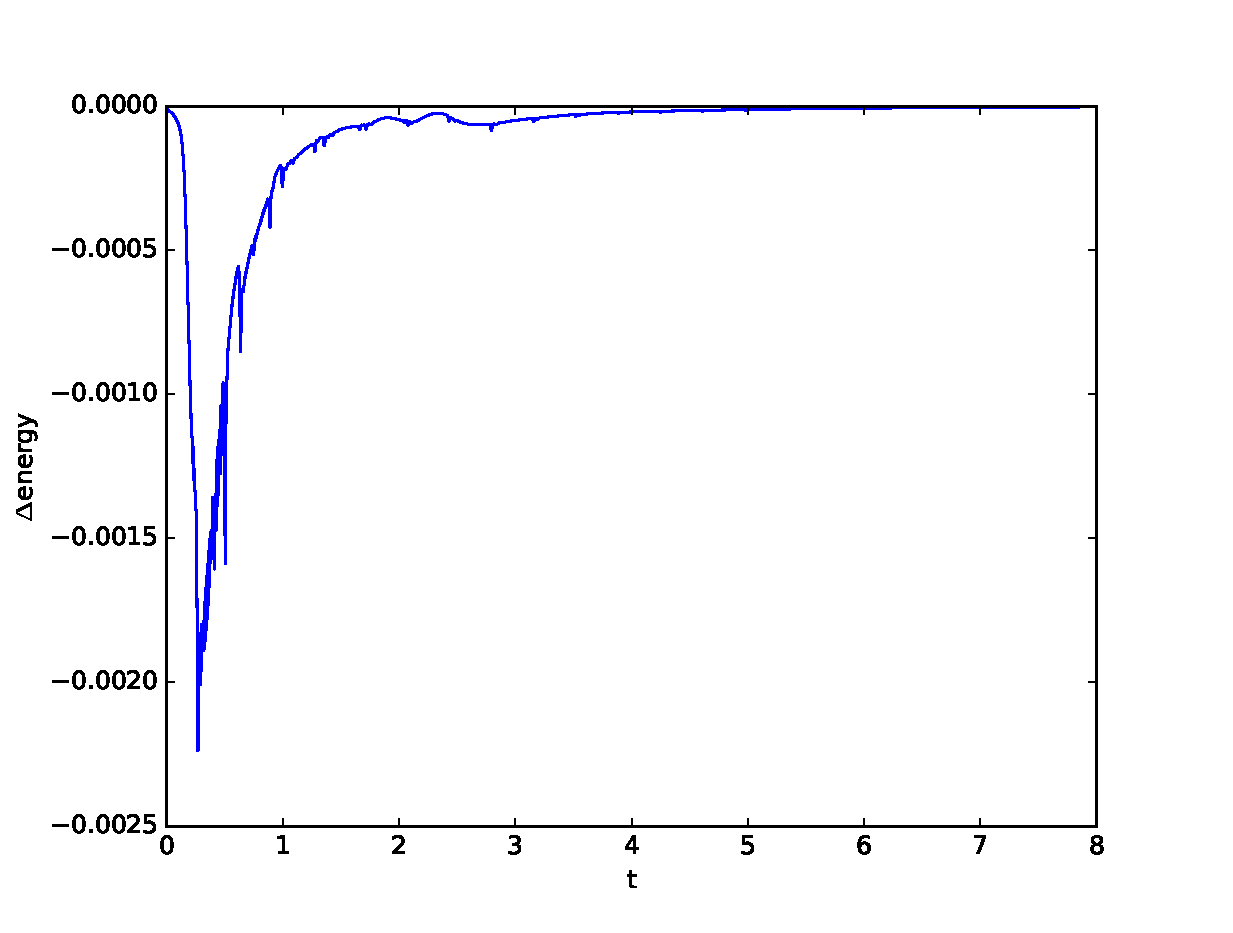
\includegraphics[width=1.1\textwidth,height=0.52\textwidth]{images/E1d.eps}\hfill
        \caption{Energy}
        \label{fig:Energy}
    \end{subfigure}
    \hfill
    \begin{subfigure}[b]{0.9\textwidth}
        \centering
        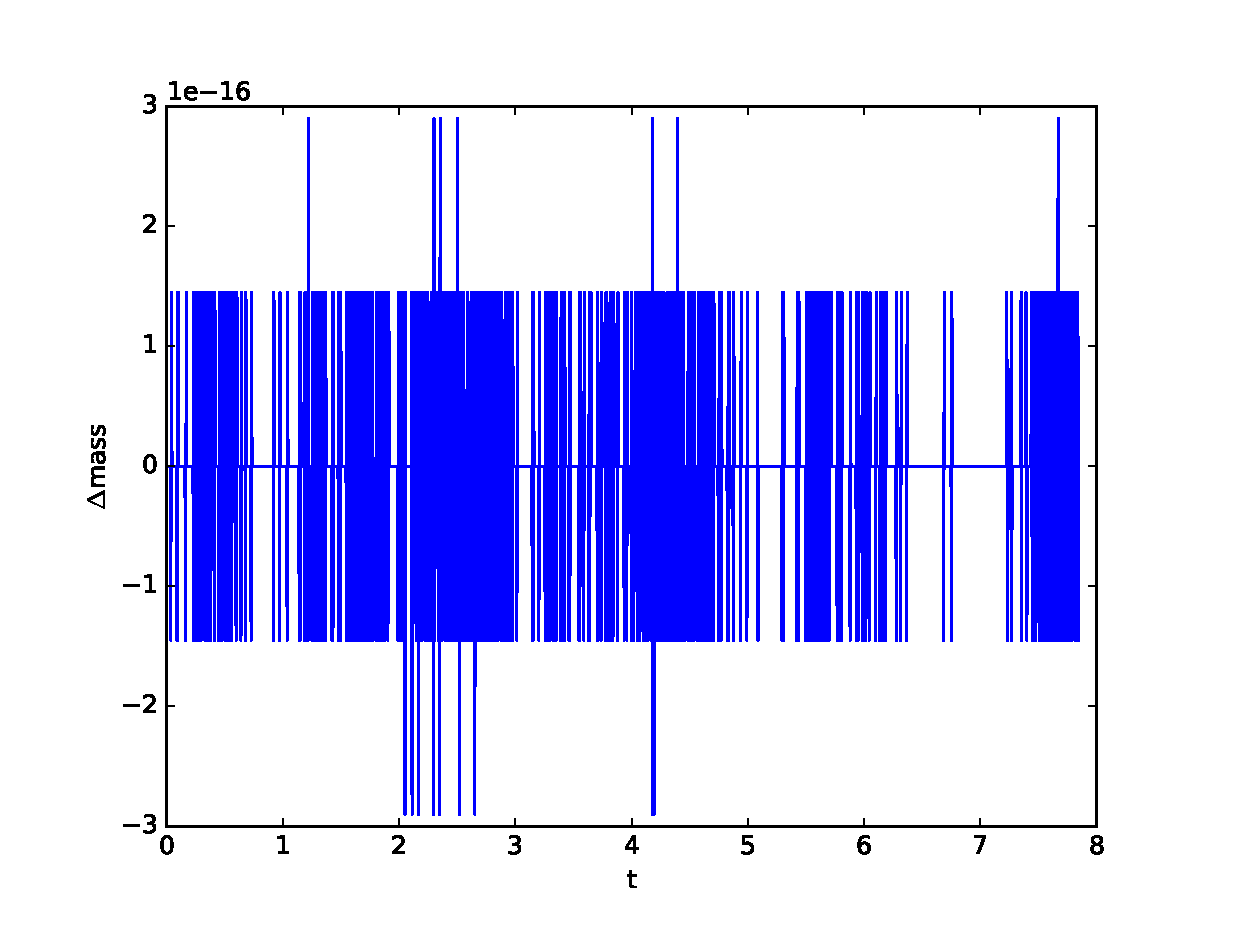
\includegraphics[width=1.1\textwidth, height=0.52\textwidth]{images/Ma1d.eps}\hfill
        \caption{Mass}
        \label{fig:Mass}
    \end{subfigure}
    \hfill
    \begin{subfigure}[b]{0.9\textwidth}
        \centering
        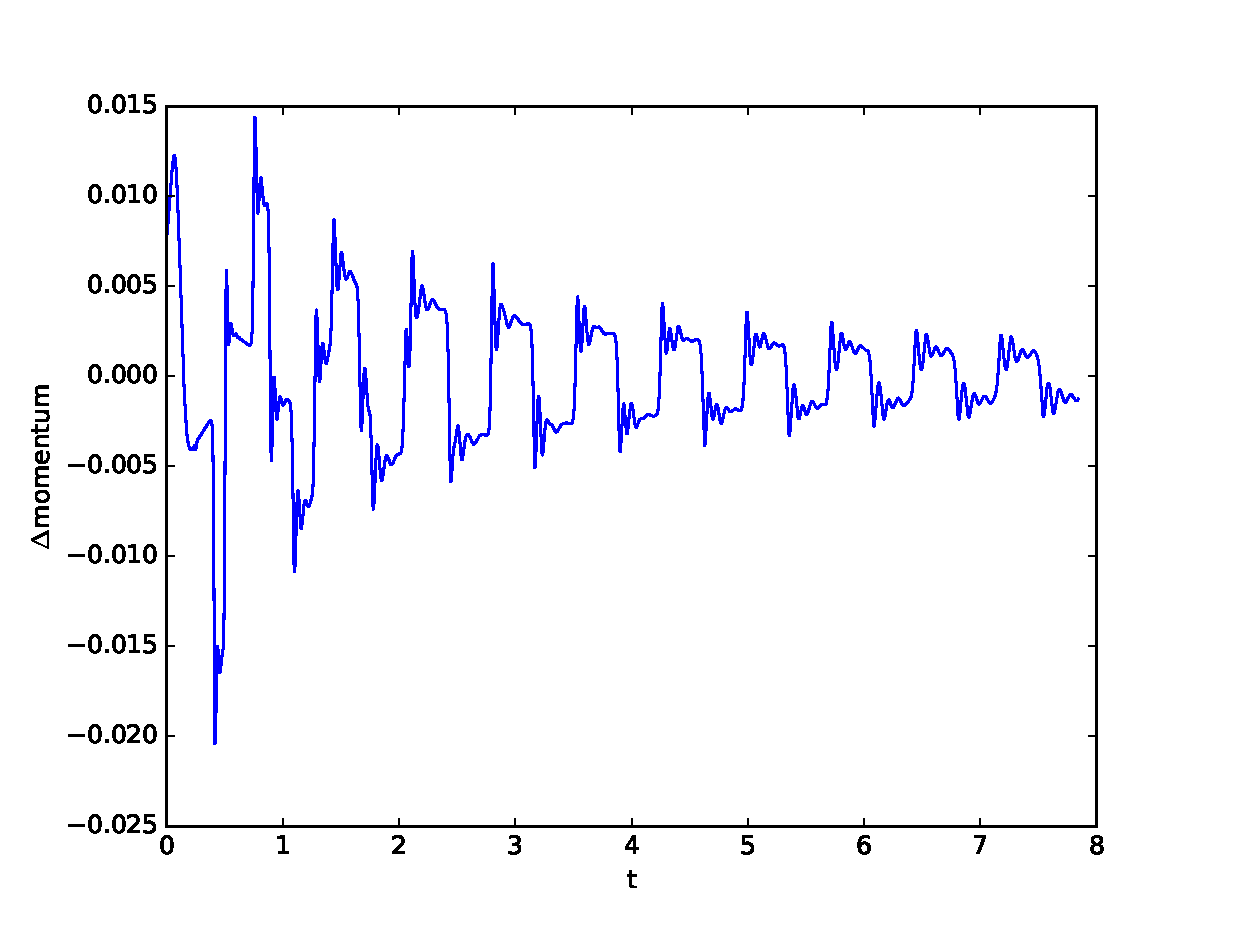
\includegraphics[width=1.1\textwidth,height=0.52\textwidth]{images/Mo1d.eps}\hfill
        \caption{Momentum}
        \label{Momentum}
    \end{subfigure}
    \caption{1D conservation plots.}
    \label{fig:1D_cons}
\end{figure}

\subsection{2D Conservation Laws}

The conservation laws in the 2D solver shows similar differences
between the conserved quantities Figure~\ref{fig:2Dcons_A}. In the 2D scheme mass, momentum and energy are hypothetically 
guessed to be strictly conserved onced again. The energy suffers from the same inherent flaws
of the numerical scheme as before, and does not initially conserve energy similar to 1D. Therefore mass,
momentum and energy are not adequetly conserved as before, which leads to the same presumption given for the 1D case. 
\newline

\begin{figure}[h!]
    \centering
    \begin{subfigure}[b]{0.9\textwidth}
        \centering
        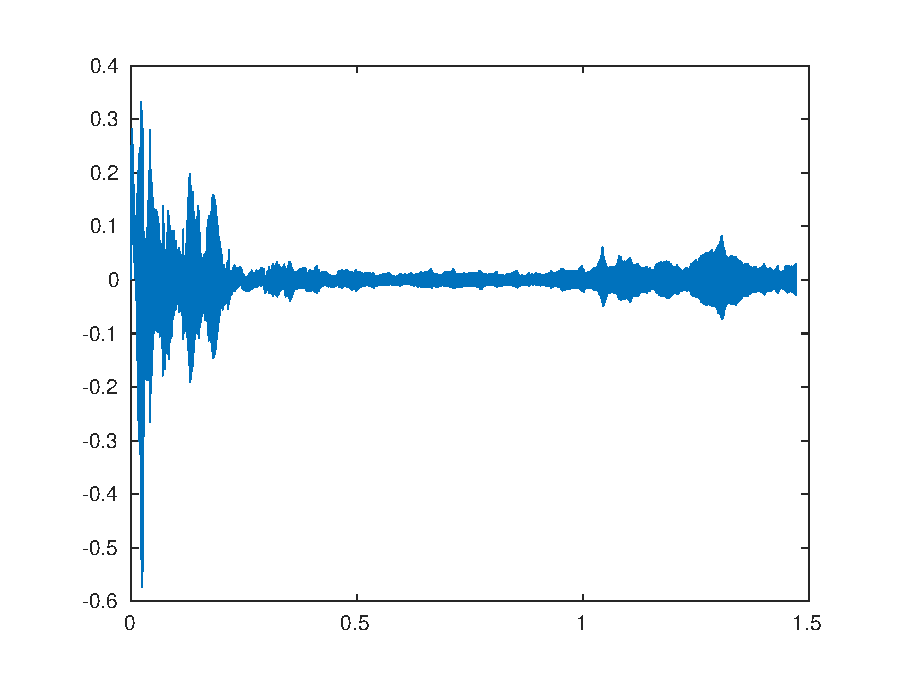
\includegraphics[width=1.1\textwidth,height=0.52\textwidth]{images/cons_energy.eps}\hfill
        \caption{Energy}
        \label{fig:Energy}
    \end{subfigure}
    \hfill
    \begin{subfigure}[b]{0.9\textwidth}
        \centering
        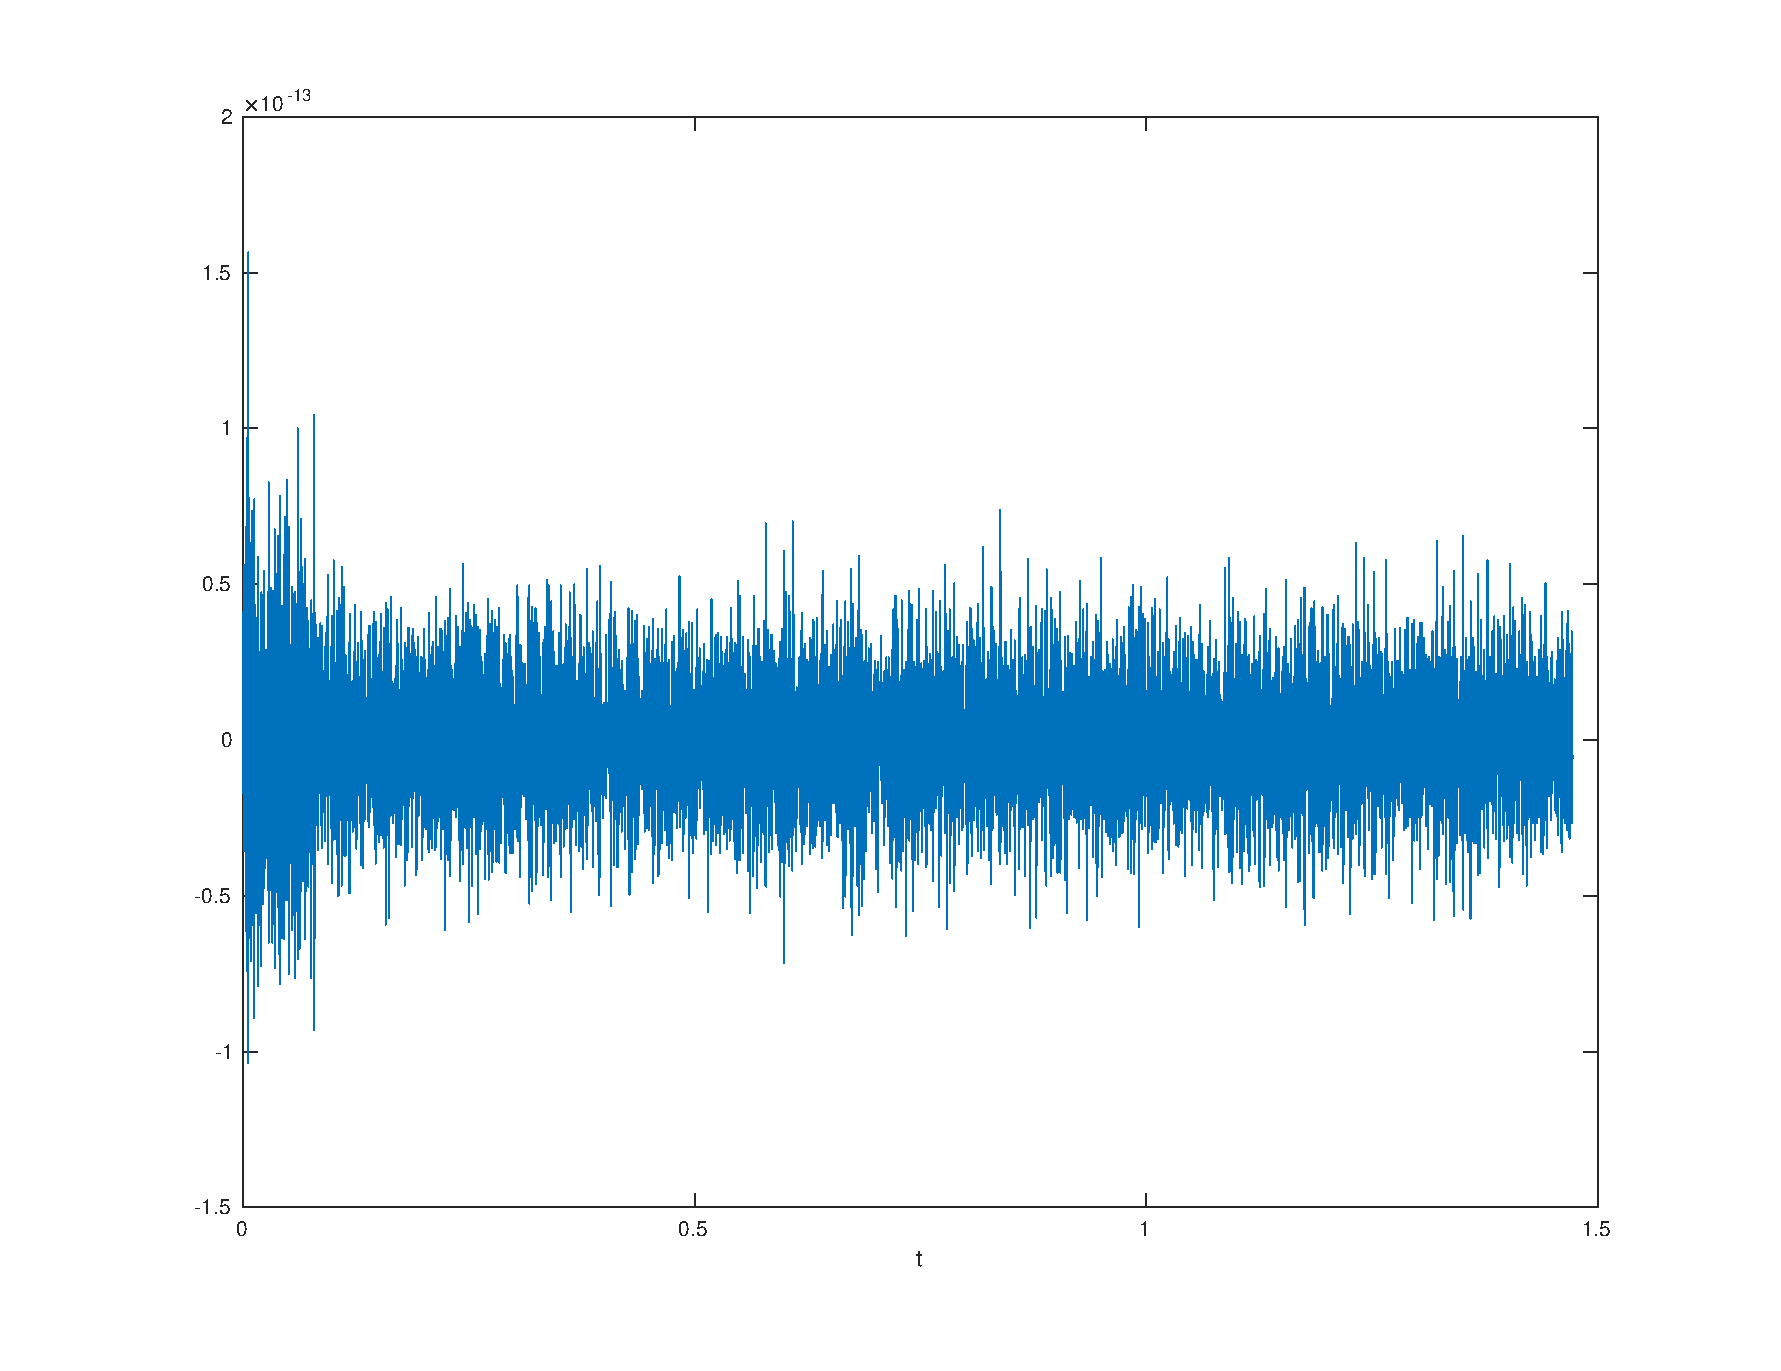
\includegraphics[width=1.1\textwidth, height=0.52\textwidth]{images/cons_mass.eps}\hfill
        \caption{Mass}
        \label{fig:Mass}
    \end{subfigure}
    \hfill
    \caption{2D conservation plots of mass and energy.}
    \label{fig:2Dcons_A}
\end{figure}


The potential vorticity given by this formula,
\begin{equation}\label{eqn:13}
\frac{\partial hv}{\partial x} - \frac{\partial hu}{\partial y} 
\end{equation}
should be conserved. We show it to be conservatived using the 2D two-step method
of Richtmeyer Figure~\ref{fig:2Dcons_B}.
\newline

\begin{figure}[h!]
    \centering
    \begin{subfigure}[b]{0.9\textwidth}
        \centering
        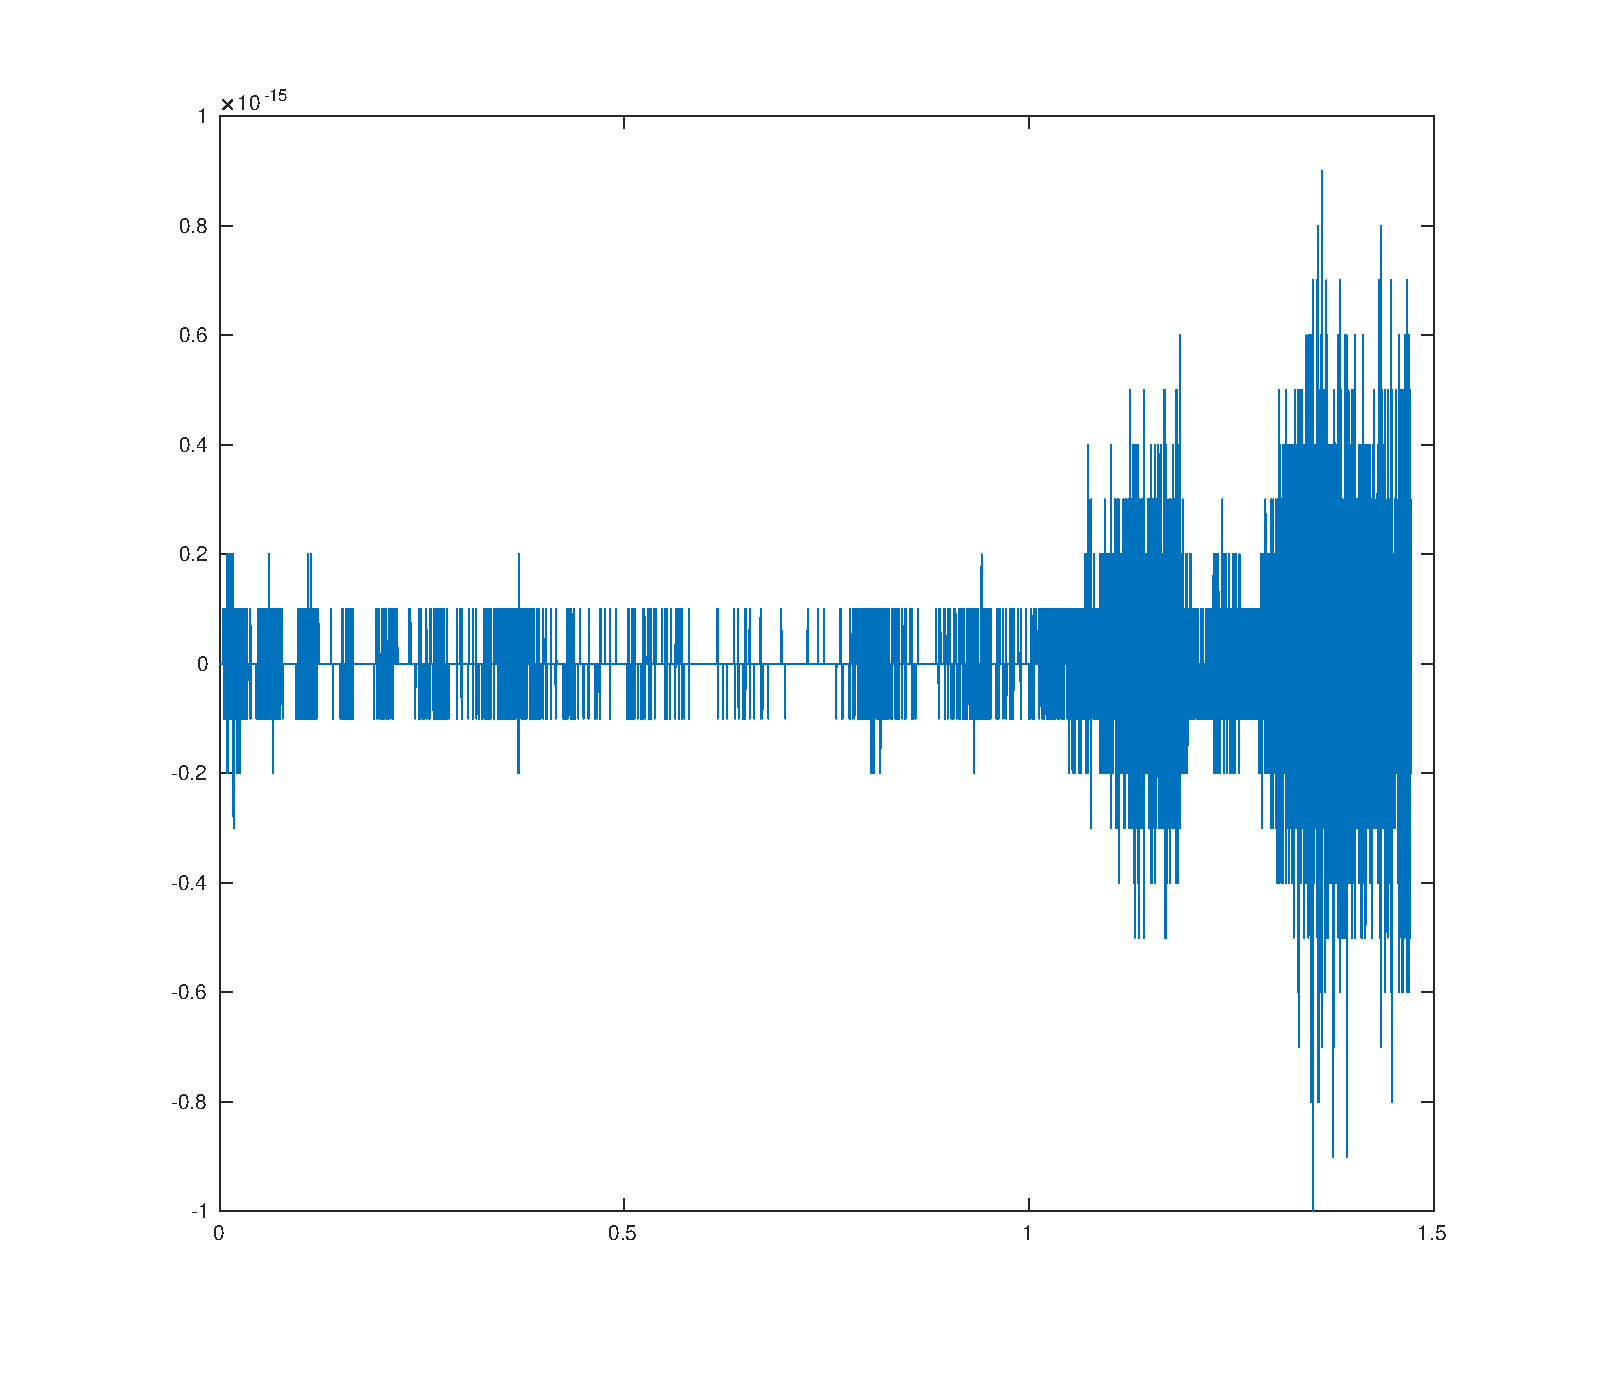
\includegraphics[width=1.1\textwidth,height=0.52\textwidth]{images/cons_momu.eps}\hfill
        \caption{u-momentum}
        \label{fig:Energy}
    \end{subfigure}
    \hfill
    \begin{subfigure}[b]{0.9\textwidth}
        \centering
        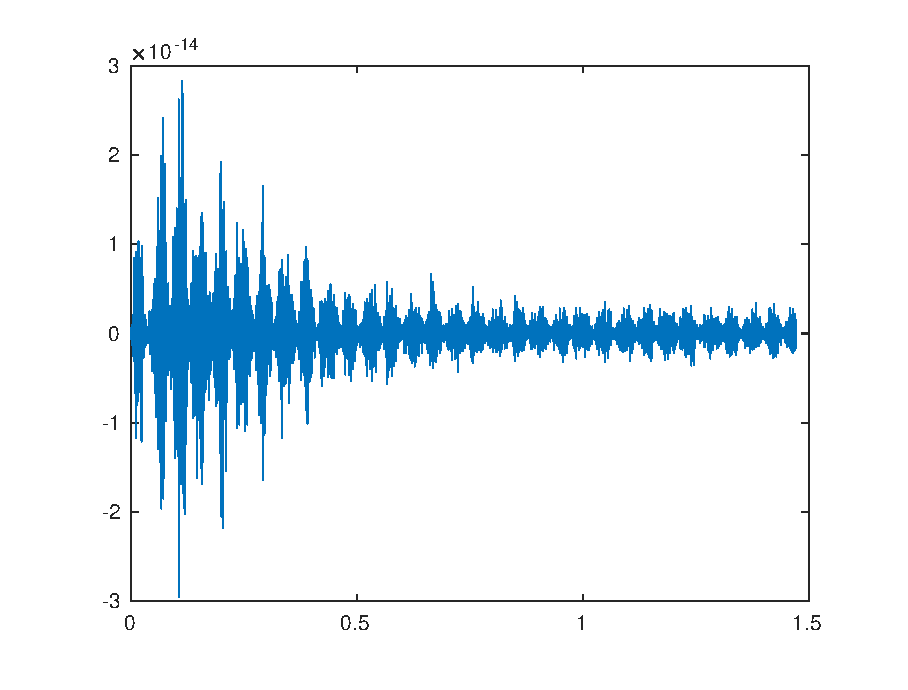
\includegraphics[width=1.1\textwidth, height=0.52\textwidth]{images/cons_momv.eps}\hfill
        \caption{v-momentum}
        \label{fig:Mass}
    \end{subfigure}
    \hfill
    \begin{subfigure}[b]{0.9\textwidth}
        \centering
        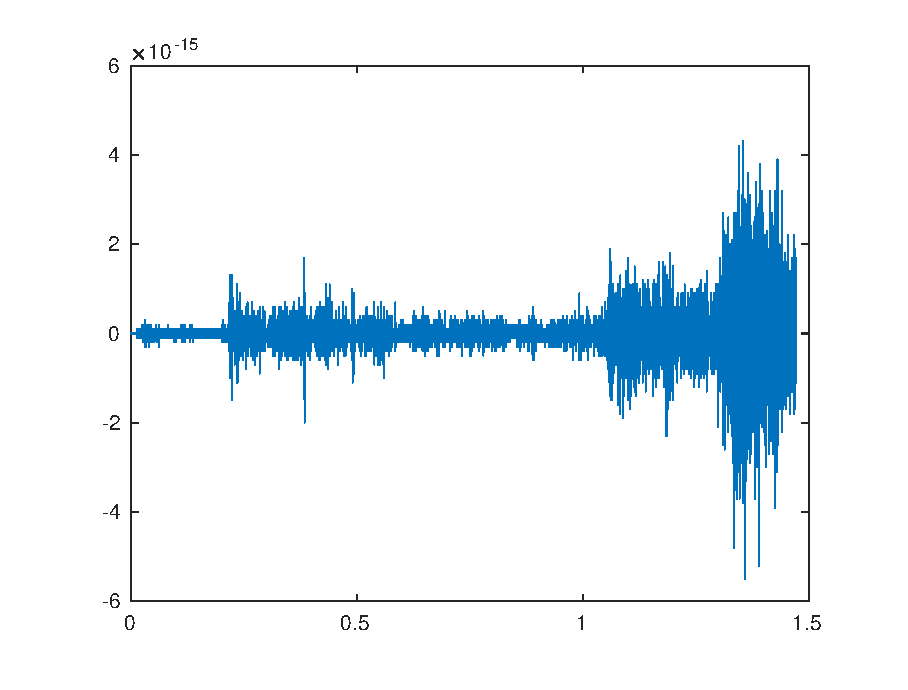
\includegraphics[width=1.1\textwidth,height=0.52\textwidth]{images/cons_vort.eps}\hfill
        \caption{vorticity}
        \label{Momentum}
    \end{subfigure}
    \caption{conservation plots of momentum, vorticity.}
    \label{fig:2Dcons_B}
\end{figure}

We draw the conlusion that the physical quantities mass, momentum and energy are not adequetly conserved due to the inability of
the applied numerical schemes due to the inability to capture the spurious oscilations produced by shocks for both the 1D and 2D methods.
Finally we have shown